\RequirePackage{lineno}
%\documentclass[aps,prl,twocolumn,superscriptaddress]{revtex4}
\documentclass[aps,prl,superscriptaddress,preprint]{revtex4}

%\usepackage[a4paper, total={7in, 9in}]{geometry}


\usepackage{graphicx,amsmath}
\usepackage{color}

\usepackage{booktabs}
\usepackage[flushleft]{threeparttable}

\usepackage{amssymb}
\usepackage{amsmath}
\usepackage{float}
\usepackage{psfrag}
\usepackage{siunitx}
\usepackage{ulem}




\renewcommand{\figurename}{Figure}

%\bibliographystyle{prsty_allauthors}

\setlength{\tabcolsep}{4pt}

\newcommand{\refe}[1]{\ref{eq:#1}} % reference to equations
\newcommand{\reff}[1]{\ref{fig:#1}} % reference to figures
\newcommand{\mar}[1]{\marginpar{\footnotesize{\textcolor{red}{#1}}}} % commentaire en marge
\newcommand{\red}[1]{{\textcolor{red}{#1}}} % commentaire en rouge
\newcommand{\blue}[1]{{\textcolor{blue}{#1}}} 
\newcommand{\green}[1]{{\textcolor{green}{#1}}} 

\def\be{\begin{equation}}
\def\ee{\end{equation}}
\def\ba{\begin{eqnarray}}
\def\ea{\end{eqnarray}}


\newcommand{\replaced}[2]{\blue{#1\sout{#2}}}
\newcommand{\deleted}[1]{\blue{\sout{#1}}}
\newcommand{\added}[1]{\blue{#1}}
\newcommand{\annotation}[1]{\blue{[\textit{#1}]}}

\renewcommand{\Re}{\operatorname{Re}}
\newcommand{\Ra}{\operatorname{Ra}}
\newcommand{\Ta}{\operatorname{Ta}}
\newcommand{\St}{\operatorname{St}}
\newcommand{\Nu}{\operatorname{Nu}_{\omega}}
\newcommand{\lam}{\operatorname{lam}}
\newcommand{\Ro}{\operatorname{Ro}}



%%% Uncomment the following lines to remove the colored highlights  %%%

%Uncomment to remove changes:
%\renewcommand{\replaced}[2]{#1} \renewcommand{\deleted}[1]{} \renewcommand{\added}[1]{}

%Uncomment to remove annotations [...]:
%\renewcommand{\annotation}[1]{}

%%%%%%%%


\begin{document}
%\linenumbers

\title{Wall-roughness induces asymptotic ultimate turbulence}
%\annotation{MANUSCRIPT FORMATTING GUIDE: Titles do not exceed two lines in print. This equates to 90 characters (including spaces) for Letters, or 75 characters (including spaces) for Articles.}} 
\author{Xiaojue Zhu } \thanks{These authors contributed equally to this work}
\affiliation{Physics of Fluids Group, MESA+ Institute and J. M. Burgers Centre for Fluid Dynamics, University of Twente, P.O. Box 217, 7500AE Enschede, The Netherlands}

\author{Ruben A. Verschoof} \thanks{These authors contributed equally to this work}
\affiliation{Physics of Fluids Group, MESA+ Institute and J. M. Burgers Centre for Fluid Dynamics, University of Twente, P.O. Box 217, 7500AE Enschede, The Netherlands}

\author{Dennis Bakhuis}
\affiliation{Physics of Fluids Group, MESA+ Institute and J. M. Burgers Centre for Fluid Dynamics, University of Twente, P.O. Box 217, 7500AE Enschede, The Netherlands}

\author{Sander G. Huisman}
\affiliation{Univ Lyon, Ens de Lyon, Univ Claude Bernard, CNRS, Laboratoire de Physique, F-69342 Lyon, France}

\author{Roberto Verzicco }
\affiliation{Dipartimento di Ingegneria Industriale, University of Rome ``Tor Vergata", Via del Politecnico 1, Roma 00133, Italy}
\affiliation{Physics of Fluids Group, MESA+ Institute and J. M. Burgers Centre for Fluid Dynamics, University of Twente, P.O. Box 217, 7500AE Enschede, The Netherlands}



\author{Chao Sun}
\email{chaosun@tsinghua.edu.cn}
\affiliation{Center for Combustion Energy and Department of Thermal Engineering, Tsinghua University, 100084 Beijing, China}
\affiliation{Physics of Fluids Group, MESA+ Institute and J. M. Burgers Centre for Fluid Dynamics, University of Twente, P.O. Box 217, 7500AE Enschede, The Netherlands}

\author{Detlef Lohse}
\email{d.lohse@utwente.nl}
\affiliation{Physics of Fluids Group, MESA+ Institute and J. M. Burgers Centre for Fluid Dynamics, University of Twente, P.O. Box 217, 7500AE Enschede, The Netherlands}
\affiliation{Max Planck Institute for Dynamics and Self-Organization, 37077 G\"ottingen, Germany}


\date{\today}

\begin{abstract} 
%\begin{linenumbers}
%\annotation{MANUSCRIPT FORMATTING GUIDE: Articles have a summary, separate from the main text, of up to 150 words, which does not have references, and does not contain numbers, abbreviations, acronyms or measurements unless essential. Some published articles also have reference in their summary. .}
Turbulence is omnipresent in Nature and technology, governing the transport of heat, mass and momentum on multiple scales. For real-world applications of wall-bounded turbulence, the underlying surfaces are virtually always rough \cite{sch00,pop00,jim04}, yet characterizing the effects of wall-roughness for turbulence in closed systems remain an elusive challenge \cite{ahl09,gro16}. By combining extensive experiments and numerical simulations of the paradigmatic Taylor-Couette system, the flow between two independently rotating concentric cylinders, we uncover the mechanism that causes the considerable enhancement of the overall transport properties by wall-roughness. If only one of the walls is rough, we reveal that the bulk velocity is slaved to the rough side, due to the much stronger coupling to that wall. If both walls are rough, the viscosity dependence is eliminated completely in the boundary layers and we thus achieve asymptotic ultimate turbulence, the upper limit of transport, whose existence had been predicted by R.\ Kraichnan in 1962 \cite{kra62}, in which the scalings laws can be extrapolated to arbitrarily large Reynolds numbers.

%\end{linenumbers}
\end{abstract}

%\pacs{47.55.D-, 66.10.C-}

\maketitle

%%%%%%%%%%%%%%%%%%%%%%%%%%%%%%%%%%%%%%%%%%%%%%%%%%%%%%%%%%%%%%%%
%%%%%%%%%%%%%%%%%%%%%%%%      MAIN TEXT           %%%%%%%%%%%%%%%%%%%%%%%%%%%%%
%%%%%%%%%%%%%%%%%%%%%%%%%%%%%%%%%%%%%%%%%%%%%%%%%%%%%%%%%%%%%%%%
%\annotation{\textbf{Section headline here?}. Nature articles typically have catchy headlines for sections.}

%\annotation{MANUSCRIPT FORMATTING GUIDE: Section 1: beginning with up to 500 words of referenced text expanding on the background to the work (some overlap with the summary is acceptable)}

\section{Introduction} 

While the vast majority of studies on wall-bounded turbulence assume smooth walls, flow boundaries are in general rough in engineering applications and the more in Nature, leading to a coupling of the small roughness scale with the much larger outer length scale of the turbulent flow. This holds for the atmospheric boundary layer over canopy or buildings, for geophysical flow, but also for many industrial flows such as pipe flow, for which the presumably most famous study on roughness was performed \cite{nik33}. For excellent reviews on the effect of wall-roughness in turbulence we refer to Ref. \cite{jim04} or textbooks such as Refs. \cite{pop00,sch00}.

The disadvantage of pipe flow studies however is that the flow is not closed and that simultaneous measurements
of local and global flow properties are difficult. This problem is overcome in Taylor-Couette (TC) flow \cite{gro16},
in which the overall torque $\tau$ to keep the cylinders at constant angular velocity is directly connected with the 
spatially averaged energy dissipation rate $\epsilon$. 
This can be expressed in terms of the friction factor 
\be
c_f = {\tau\over  \ell \rho_f \nu^2 (\mathrm{Re}_i-\eta \mathrm{Re}_o)^2}= {\pi \eta \over (1-\eta)}    {\epsilon\over (U_i-\eta U_o)^3/(r_i+r_o) } . 
\label{tau-eps}
\ee
Here
$U_{i,o}$ are the velocities of the inner resp. outer 
cylinder, $r_{i,o}$  their radii, $\nu$ the kinematic viscosity (together defining the
inner and outer Reynolds numbers $\mathrm{Re}_{i,o} = U_{i,o} d/\nu$), $\rho_f$ the density of the fluid, $\ell$ the height of the TC cell,
$d=r_o-r_i$ the gap width, 
and $\eta =  r_i/r_o$ the ratio between outer and inner cylinder radius. 
The key question now is: how does the friction factor $c_f$ depend on the (driving) Reynolds number $Re_{i}$ and
how does wall-roughness affect this relation?

Alternatively, the relation $c_f$ can be expressed as a ``Nusselt number'' $\mathrm{Nu}_\omega$ \cite{eck07b}, where 
$\mathrm{Nu}_\omega =  \tau / (2\pi \ell \rho_f  J_{lam}^\omega )$ with 
$J^\omega_{lam} = 2\nu r_i^2 r_o^2
(\omega_i - \omega_o)/ (r_o^2 - r_i^2)$ 
depending on 
the Taylor number 
$\Ta= \frac{1}{64}\frac{(1+\eta)^4}{\eta^2} d^2 (r_i+r_o )^2(\omega_i - \omega_o)^2\nu^{-2}$ \cite{gro16}, 
with $\omega_{i,o}$ the angular velocity of the inner resp.\ outer cylinder. 
This notation $\mathrm{Nu}_\omega (\mathrm{Ta})$ stresses the analogy between TC flow and Rayleigh-B\'enard flow (RB) \cite{ahl09,loh10},
the flow in a box heated from below and cooled from above, 
where the Nusselt number $\mathrm{Nu}$ (the dimensionless heat flux) depends  on the Rayleigh number $\textrm{Ra}$ (the dimensionless
temperature difference). For that system Kraichnan \cite{kra62} had postulated an ultimate scaling regime 
\be
\mathrm{Nu} \sim \mathrm{Ra}^{1/2} (\log \mathrm{Ra} )^{-3/2} 
\label{kra-rb1}
\ee
(for fixed Prandtl number). 
 In analogy, such an ultimate regime should also exist for TC flow,
 namely 
 \be
\mathrm{Nu}_\omega \sim \mathrm{Ta}^{1/2} (\log \mathrm{Ta} )^{-3/2}, 
\label{kra-tc1}
\ee
 as worked out in Ref.\ 
 \cite{gro11}. 
 In fact, in that  reference slightly different log-dependences were derived, namely 
 \begin{eqnarray} \label{kra-rb2}
 \mathrm{Nu} & \sim &  \mathrm{Ra}^{1/2} {\cal{L}}(\mathrm{Re}),  \quad \hbox{and}\\
 \mathrm{Nu}_\omega & \sim &  \mathrm{Ta}^{1/2} {\cal{L}}(\mathrm{Re}),
 \label{kra-tc2} 
 \end{eqnarray}
 where ${\cal{L}} (\mathrm{Re} (\mathrm{Ra}))$ resp.
 ${\cal{L}} (\mathrm{Re} (\mathrm{Ta}))$ 
 are logarithmic dependences (see Methods and also Ref.\  \cite{gro11}).  
 Irrespective of whether one takes the logarithmic dependences 
 (\ref{kra-rb1}) resp.\ 
 (\ref{kra-tc1}) or 
   (\ref{kra-rb2}) resp.\ 
 (\ref{kra-tc2}), for smooth walls 
 due to these log-corrections 
 the {\it effective} scaling exponent for the largest experimentally achievable 
 Rayleigh (Taylor) numbers is only around 0.38 and not 1/2, i.e., $\mathrm{Nu}\sim \mathrm{Ra}^{0.38}$ resp. $\mathrm{Nu}_\omega\sim \mathrm{Ta}^{0.38}$. 
 This effective exponent 0.38 has indeed been observed in large $\mathrm{Ra}$ RB experiments \cite{he12,he12a} 
and large $\mathrm{Ta}$ TC experiments \cite{hui12,gro16} and numerical simulations \cite{ost14pd,gro16}. 
The log-corrections, which are intimately connected with the logarithmic boundary layers \cite{ost16jfm}, thus
prevent the observation of the asymptotic ultimate regime exponent $1/2$. This exponent has only been achieved in 
artificial configurations, such as numerical simulations of so-called ``homogeneous  turbulence'' \cite{loh03} with periodic
boundary conditions and no boundary layers or experimental realisations thereof such as in ref.\ \cite{gib06,cho09}. The asymptotic exponent $1/2$ in the $\mathrm{Nu}$ vs. $\mathrm{Ra}$ resp. $\mathrm{Nu}_\omega$ vs. $\mathrm{Ta}$ scaling law corresponds to a friction factor $c_f$ being {\it independent} on the Reynolds number. Vice versa, in the friction factor the logarithmic dependences of eqs.\ (\ref{kra-rb1}) to (\ref{kra-tc2}) are expressed in the so-called Prandtl-von K\'arm\'an skin friction law, i.e.\ $1/\sqrt c_f = a \mathrm{log}_{10} (\Re_i \sqrt c_f) + b$ \cite{kar21,sch00,pop00}, which can be obtained by assuming that the boundary layer 
  profiles at each cylinder wall are 
  logarithmic  \cite{hui13,ost14pof}. Here $a$ and $b$ are fitting constants
  connected with the von K\'arm\'an constant $\kappa$. 
 
 
 
 How to get rid of the log-correction and to thus achieve asymptotic ultimate turbulence with a 1/2 power law 
 or equivalently a Reynolds number independent friction factor? The path we will follow here is to introduce wall roughnnes. By combining direct numerical simulations (DNS) and experiments (EXP), we explore five decades of $\mathrm{Ta}$ to present conclusive evidence that the 1/2 power law can be realized, thus achieving the asymptotic ultimate regime. Moreover, we will give a theoretical justification for the
 findings based on measurements of the global and local flow structures and extend the analysis also to outer cylinder rotation. 
 
 
  \begin{figure}[!h]
\begin{center}
\includegraphics[height=4.0in]{1.eps}
\caption{
{\bf Plume structures for smooth and rough Taylor-Couette turbulence.} Here the volume renderings of azimuthal velocity at $\Ta=2.15\times10^9$ are shown, from numerical simulations. {\bf a,} Both cylinders are smooth. We see that plumes are generated on both cylinders and form the structure of Taylor rolls. The plumes are concentrated in local regions and can not reach the other cylinder. {\bf b,} Both cylinders are rough. Even in the rough case, Taylor rolls still exist. We see the plumes are also generated on top of the rough element and elongate to the other cylinder, and the arrows in the top-down views illustrate the directions of plumes. All plots share the same colormap.}
\label{fig:fig1}
\end{center}
\end{figure}

 
Four cases will be considered: SS, SR, RS, and RR, where the first (second) letter specifies the configuration of the inner (outer) cylinder, which can be either rough (R) or smooth (S). In both DNS and EXP, the radius ratio between the two cylinders is $\eta=0.716$. The cylinders were made rough by attaching six vertical ribs with a square cross-section over the entire height on none, both or either one of the
cylinders (see Methods section). The roughness heights employed are much larger than the
boundary layer thickness. 
To give the reader an impression of the flow organization, 
 typical flow structures of a smooth case and a rough case are shown  in Figs.\ \ref{fig:fig1}a,b, respectively.


%\annotation{Reference information from ``manuscript formation guide': \ \\
%Articles are original reports whose conclusions represent a substantial advance in understanding of an important problem and have immediate, far-reaching implications. They do not normally exceed 5 pages of Nature and have no more than 50 references. (One page of undiluted text is about 1,300 words.) \ \\
%Articles have a summary, separate from the main text, of up to 150 words, which does not have references, and does not contain numbers, abbreviations, acronyms or measurements unless essential. It is aimed at readers outside the discipline. This summary contains a paragraph (2-3 sentences) of basic-level introduction to the field; a brief account of the background and rationale of the work; a statement of the main conclusions (introduced by the phrase 'Here we show' or its equivalent); and finally, 2-3 sentences putting the main findings into general context so it is clear how the results described in the paper have moved the field forwards. \ \\
%Articles are typically 3,000 words of text, beginning with up to 500 words of referenced text expanding on the background to the work (some overlap with the summary is acceptable), before proceeding to a concise, focused account of the findings, ending with one or two short paragraphs of discussion. \ \\
%The text may contain a few short subheadings (not more than six in total) of no more than 40 characters each (less than one line of text in length). Articles typically have 5 or 6 display items (figures or tables).}







%%%%%%%%%%%%%%%%%%%%%%%%%%%%%%%%%%%%%%%%%%%%%%%%%%%%%%%%%%%%%%%%
%%%%%%%%%%%%%%%%%%%%%%%%      MAIN TEXT  Figure1-6         %%%%%%%%%%%%%%%%%%%%%%%%
%%%%%%%%%%%%%%%%%%%%%%%%%%%%%%%%%%%%%%%%%%%%%%%%%%%%%%%%%%%%%%%

 
 
 %%%%%%%%%%%%%%%%%%%%
%%%%%% Torque scaling %%%%	
%%%%%%%%%%%%%%%%%%%%










\section{Global scaling relations} 

We first address the question of how roughness changes the global scaling relations. The global dimensionless torques, $\Nu \sim \Ta^{\gamma}$, for the four cases, with increasing $\Ta$ and fixed outer cylinder, are shown in Fig.\ \ref{fig:fig2}a. Combining EXPs and DNSs, the range of Taylor number studied here extends five decades. Similar to what has been shown in various studies recently \cite{he12,gil11,ost14pof,ost14pd,lat92,bra13}, for the SS case, an effective scaling of  $\Nu \sim \Ta^{0.38\pm0.02}$ is observed in the DNS, corresponding to the ultimate regime with logarithmic corrections \cite{kra62,gro11}. Very similar scaling exponent $\Nu \sim \Ta^{0.39 \pm 0.01}$ is found in EXP, demonstrating the excellent agreement between DNS and EXP. Dramatic enhancements of the torques are clearly observed with the introduction of wall-roughness, resulting in the transition of $\Nu$ from $\mathcal{O}(10^2)$ to $\mathcal{O}(10^3)$. Specifically, when only a single cylinder is rough, the logarithmic corrections reduce and the scaling exponents marginally increase, implying the scaling in the 
flow is dominated by the single smooth wall. For the RR case, best fits of $\Nu \sim \Ta^{0.50\pm0.02}$ are obtained both numerically and experimentally, suggesting that the logarithmic corrections are canceled and the asymptotic ultimate scaling $1/2$ is seen. The compensated plots of insets of $\Nu/\Ta^{\gamma}$ show the robustness and the quality of the scalings. 

When expressing the relation between the global transport properties and the driving force in terms of
 the Reynolds number dependence of the friction factor $c_f$ we obtain  Fig.~\ref{fig:fig2}b. 
 For the SS case, the fitting parameters $a$ and $b$ yield a von K\'arm\'an constant $\kappa=0.44\pm0.01$, which is slightly larger than the standard value of 0.41 due to the curvature effect \cite{hui13,ost16jfm,bra13b}. This agrees  very well with the previous measurements on TC with smooth walls \cite{lew99}. For the RR case, in both DNS and EXP, 
 the friction factor $c_f$ is found to be independent on $\Re_i$, namely $c_f=0.29$ in the DNS and $c_f=0.23$ in the EXP. The discrepancy is caused by the implementation of different heights of riblet in DNS (10\% of the cylinders gap width) and EXP (7.5\% of the cylinders gap width). If we use the same 10\% gap width riblet in DNS, we find $c_f=0.23$. The results here are consistent with the asymptotic ultimate regime scaling $1/2$ for $\Nu$ and indicate that the Prandtl-von K\'arm\'an log-law of the wall \cite{sch00} with wall-roughness is also independent of $\Re_i$ \cite{nik33}, which has been verified recently for Taylor-Couette flow \cite{zhu17}. Note that in pipe flow, the same Reynolds number independent friction factor with wall-roughness is observed \cite{sch00,pop00}. For the RS and SR cases, one boundary is rough and the other is smooth such that the friction law lies in between RR and SS lines.     

\begin{figure}[!h]
\begin{center}
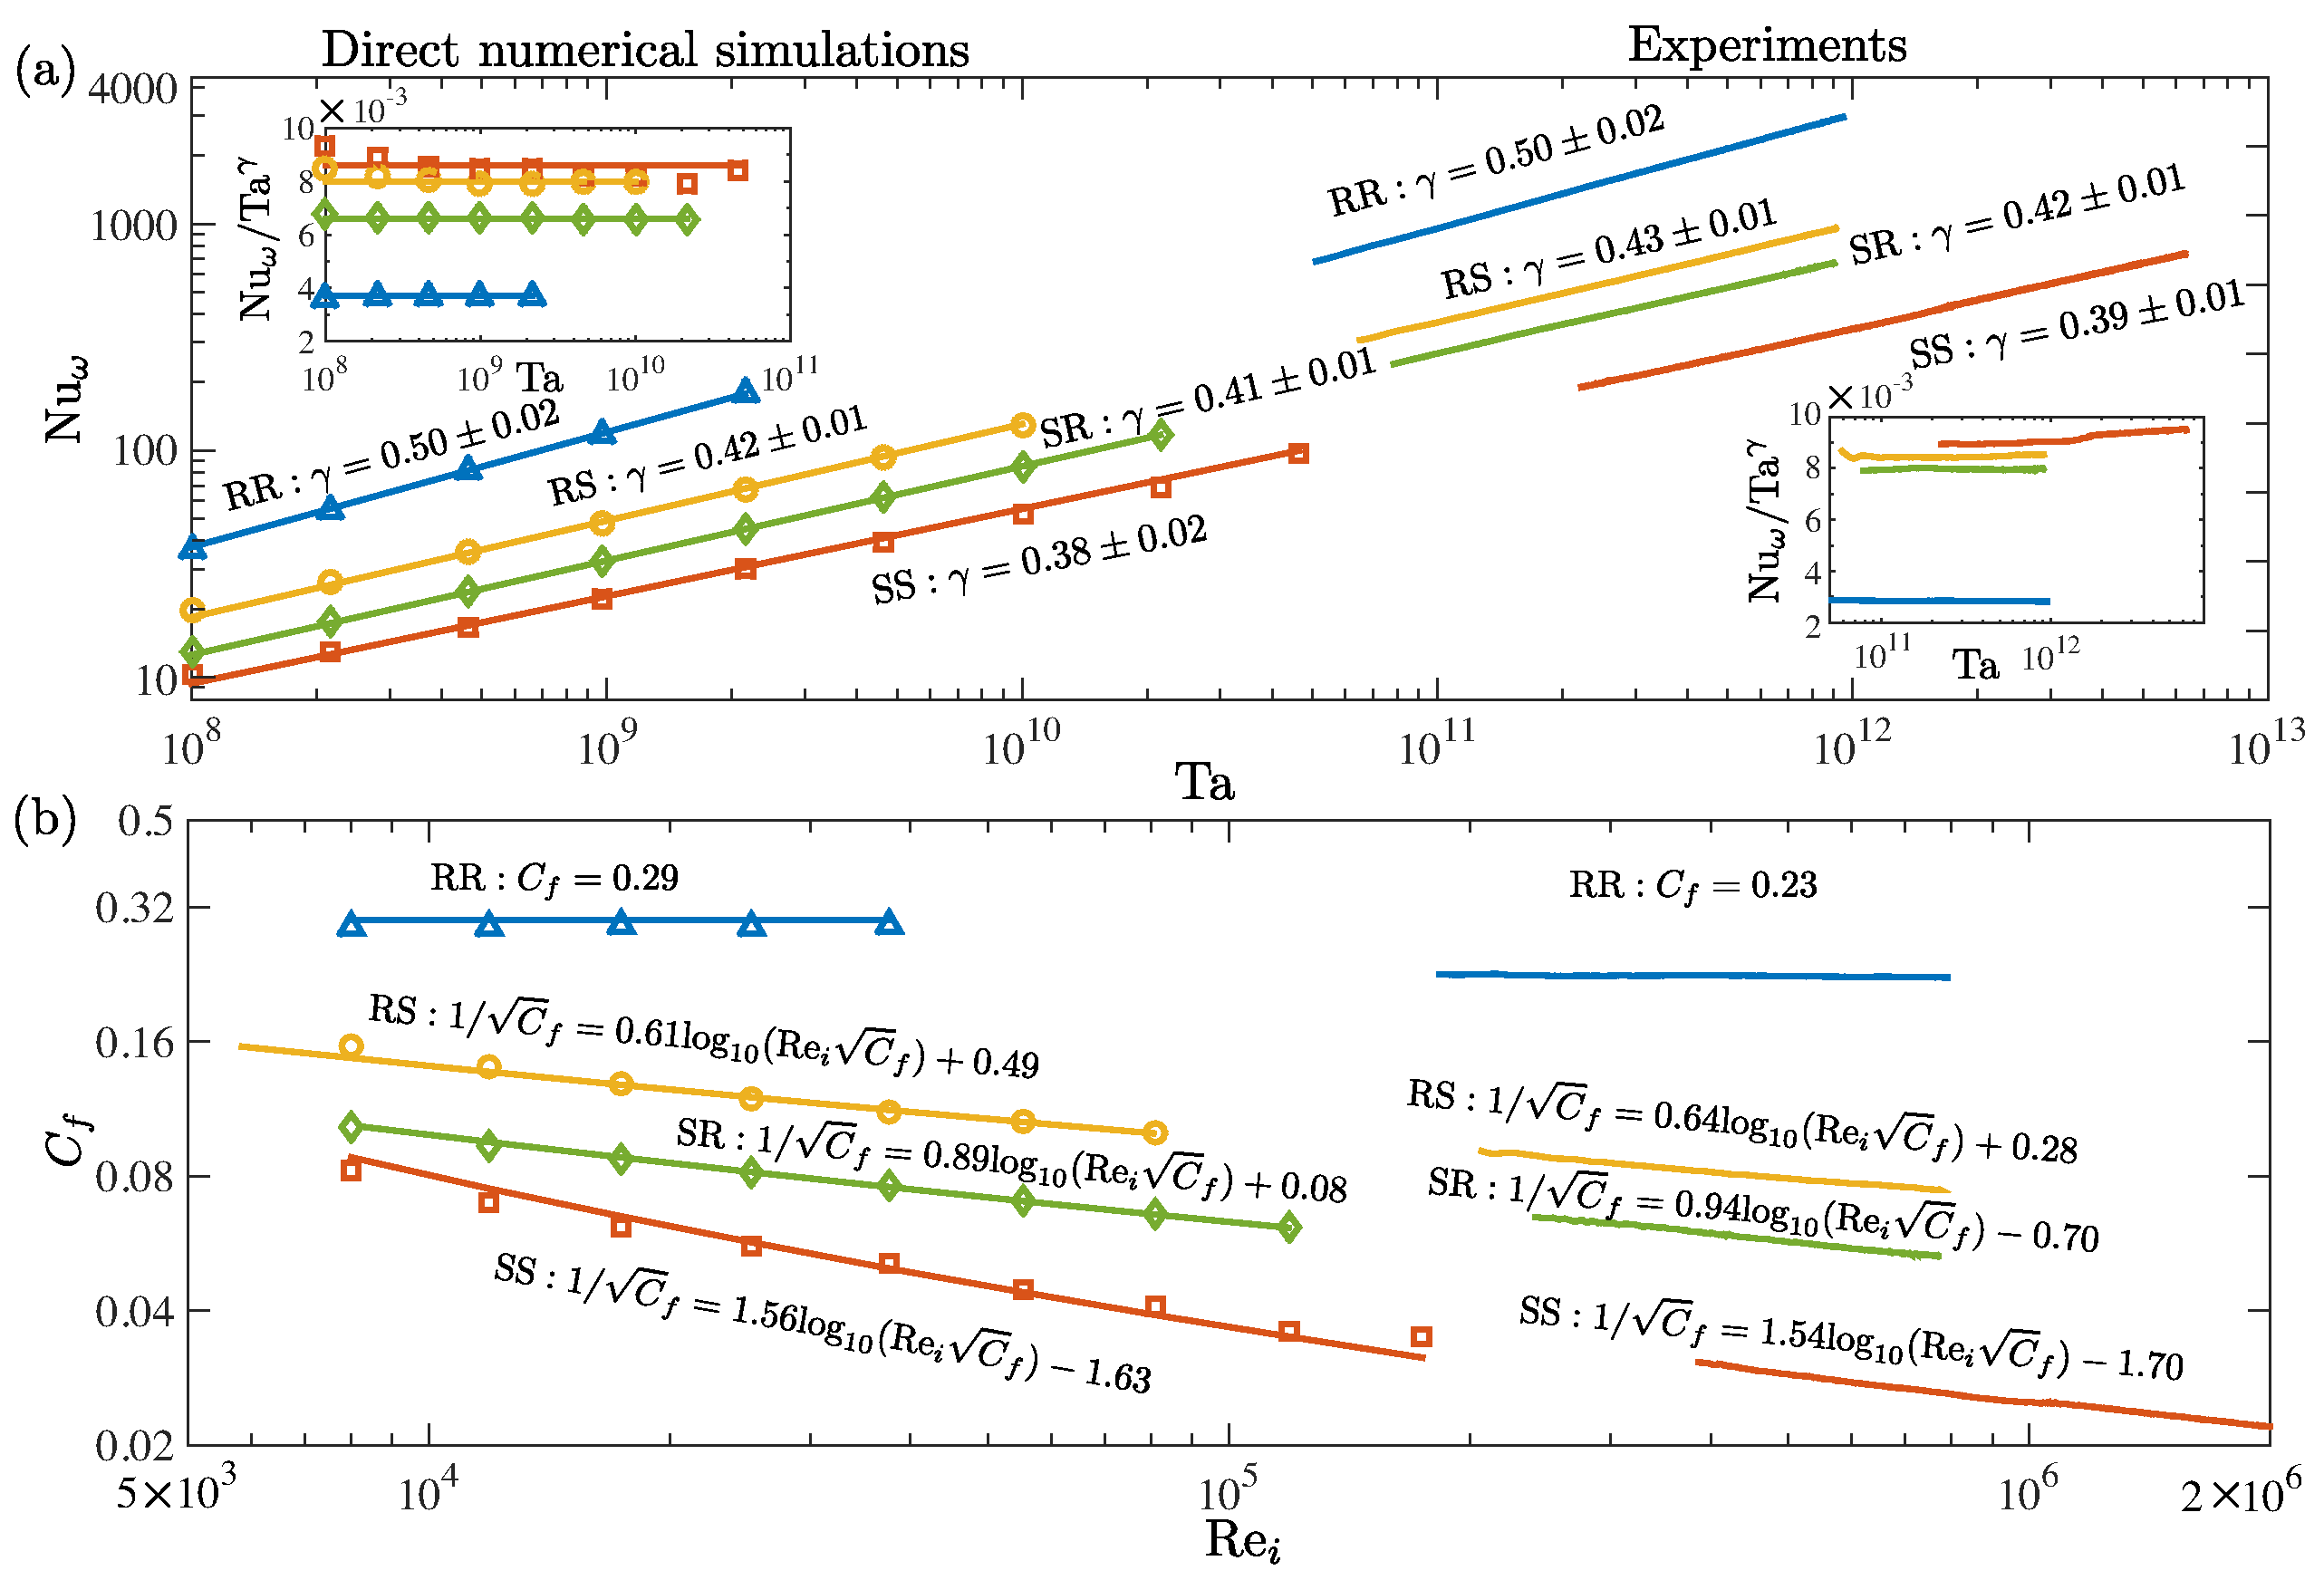
\includegraphics[width=6.4in]{2.eps}
\caption{ 
{\bf Global torque and friction factor scalings.} {\bf a,} The dimensionless torque as a function of Taylor number $\Ta$: DNS (left part), and experiments (right part). Four cases are shown: (SS) both cylinders rough; (SR) smooth inner, rough outer; (RS) rough inner, smooth outer; and (RR) both cylinders rough, with the exponent $\gamma$ in the power law relation $\textrm{Nu}_\omega \sim \mathrm{Ta}^\gamma$ shown for every case. The inset depicts the compensated plots $\Nu/\Ta^\gamma$, showing the quality of the scaling. {\bf b,} The friction factor $c_f$ as a function of the inner cylinder Reynolds number $\Re_i$: DNS (left part), and experiments (right part). The lines show the best fits of the Prandtl friction law $1/\sqrt c_f=a \mathrm{log} _{10}(\Re_i \sqrt c_f)+b$, with all prefactors shown in the figures. For RR case, $\Re_i$ independent friction factors ($c_f=0.29$ (DNS) and $c_f=0.23$ (EXP)) are revealed.
}
\label{fig:fig2}
\end{center}
\end{figure}

We now interpret the torque scalings through an extension of the Grossmann-Lohse (GL) theory \cite{gro11}, by accounting for Prandtl-von K\'arm\'an log-law of the wall \cite{sch00} in the presence of roughness. To show how this theory works, we take the example of only inner cylinder rotation. For a smooth wall, the energy dissipation rate in the log region scales with $\epsilon_{u} d^4/\nu^3 \sim \Re_i^3(u_\tau/U)^3 \mathrm{ln} (\Re_i u_\tau/U)$, which stems from the integration of the Prandtl-von K\'arm\'an log-law of the wall, where $u_\tau$ is the friction velocity and $U$ the velocity of inner cylinder. The log term in the law is dependent on $\Re_i$, which is the origin of the logarithmic correction term ${\cal{L}}(\Re)=(u_\tau/U)^3 \mathrm{ln} (\Re_i u_\tau/U)$ besides the asymptotic ultimate regime scaling $\epsilon_ud^4/\nu^3 \sim \Re_i^3$ and thus decreases the effective scaling exponent. However, with roughness, the log term in the law of the wall is independent of $\Re_i$  \cite{zhu17}, which correspondingly renders this correction \textit{constant}. Therefore, by linking the energy dissipation rate $\epsilon_{u}$, Reynolds number $\Re_i$ with the dimensionless torque $\Nu$ and driving force $\Ta$ \cite{eck07b}, the effect of logarithmic term on the scaling vanishes and asymptotic ultimate scaling $\Nu \sim \Ta^{1/2}$ emerges; see Methods for details.






%\begin{figure}[!h]
%\begin{center}
%\includegraphics[scale=.5]{new_figures/2d.eps}
%\includegraphics[scale=.5]{new_figures/2c.eps}
%\caption{ {\bf Friction factor.} The friction factor $C_f$ as a function of the inner cylinder Reynolds number $\Re_i$: experiments ({\bf a}), and DNS ({\bf b}).  The symbols are  the same as in Fig. \ref{fig2}. The lines show the best fits of the Prandtl friction law $1/\sqrt C_f=a \mathrm{log} _{10}(Re_i \sqrt C_f)+b$, with $a = 1.81$, $b =-1.43$ for SS cases, $a = 0.67$, $b = 0.56$ for RS cases. For RR case, a $Re_i$ independent $C_f=0.029$ is revealed.}
%\label{fig:cf}
%\end{center}
%\end{figure}




In a TC system, the inner and outer cylinders can rotate independently, resulting in the rotation ratio between the two cylinders $a=-\omega_o/\omega_i$ as another important parameter. 
Also with rough walls the $\Nu \sim \Ta^{\gamma}$ scalings are independent of rotation ratio, the same for the smooth wall cases \cite{gil11}. For long, it has been known that inner cylinder rotation has a destabilizing effect on the flow, whereas outer cylinder rotation has a stabilizing effect \cite{tay23b}. For TC flow with smooth walls, it was found that the optimal transport rotation ratio $a_{opt}$ between the two cylinders, where the torque reaches the maximum for a specific driving $\Ta$, is around 0.36 \cite{hui14,vee16b} instead of zero. Later it was verified that this is attributed to the existence of the strong Taylor rolls between the counter-rotating cylinders when $a<a_{opt}$. Only for strong enough counter-rotation ($a>a_{opt}$) does the stabilization through the counter-rotating outer cylinder take over \cite{gil12}. Here, we focus on whether this optimal transport rotation ratio shifts or stays the same in the presence of roughness. The results are shown in figure \ref{fig:Nu_a}. 
We find that when either one of the cylinders is rough, the effect of that rough cylinder is enhanced. 

In the SR case, little outer cylinder rotation is necessary to stabilize the flow efficiently with the help of the roughness elements. In contrast, a rough inner cylinder is much more effective to enhance the momentum transport. The optimal transport peak for the RS case occurs at larger rotation ratios, as a high outer cylinder rotation is needed to suppress turbulence originating from the inner cylinder. In this case the stabilizing effect of the smooth outer cylinder becomes inefficient. 
%Apparently, roughness couples the bulk more efficiently to the rough cylinder. 
In the RR case, the effects of the inner cylinder and outer cylinder are balanced in a similar way as in the SS case, resulting in the similar values of $a_{opt}$ found in the SS case. At optimal rotation ratio $a_{opt}$, the enhanced shear is caused by Taylor rolls \cite{hui14,ost14pd,mar14,vee16b}. This indicates that even with the presence of roughness, Taylor rolls still exist, as visible in Fig.\ \ref{fig:fig1}.




\begin{figure}[!htp]
\begin{center}
   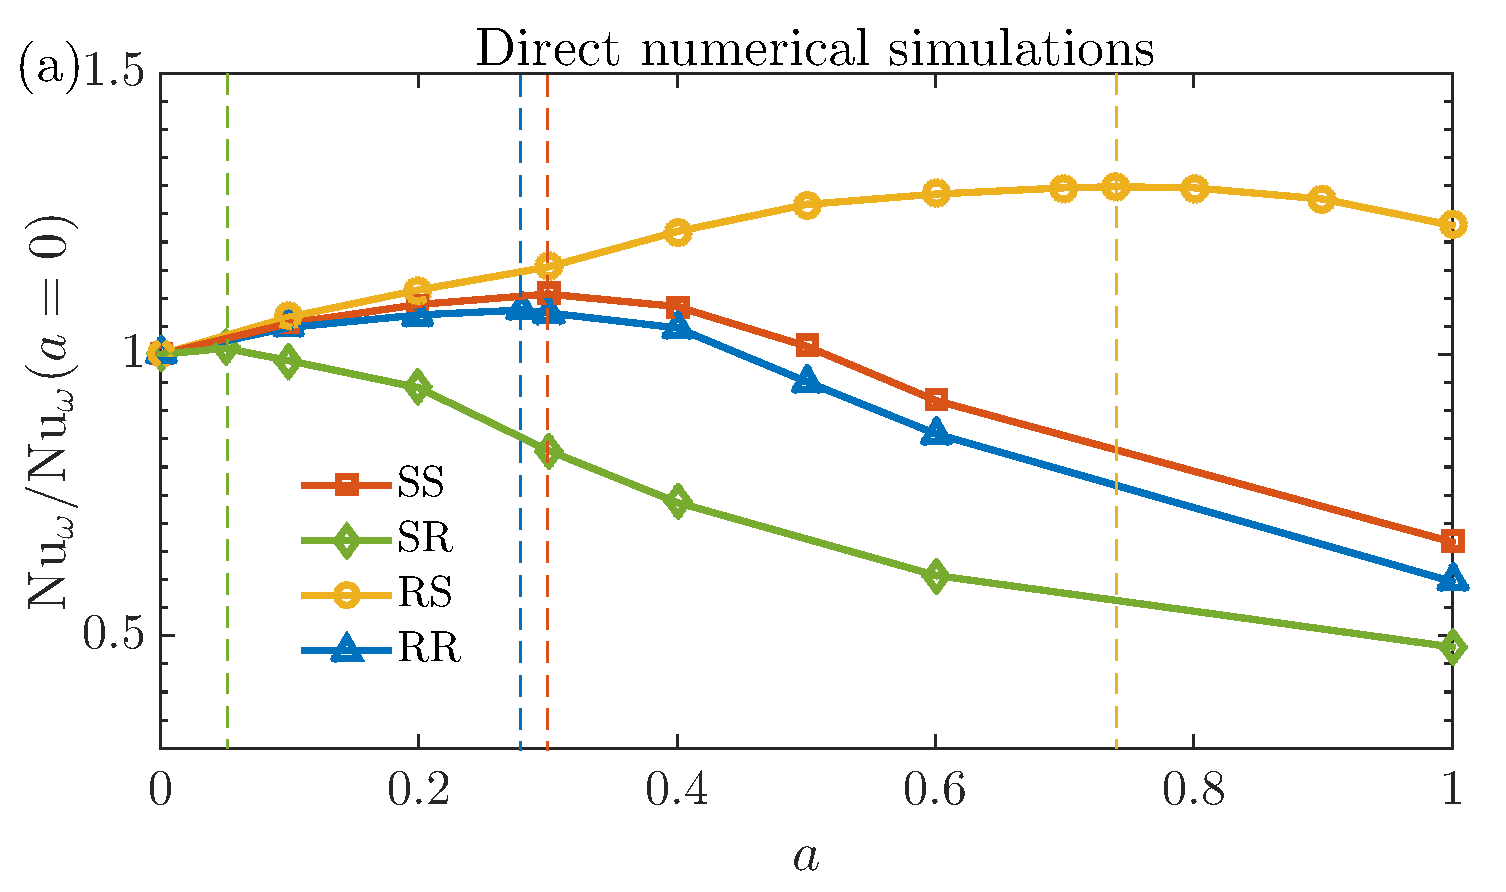
\includegraphics[width=3.2in]{3a.eps}
    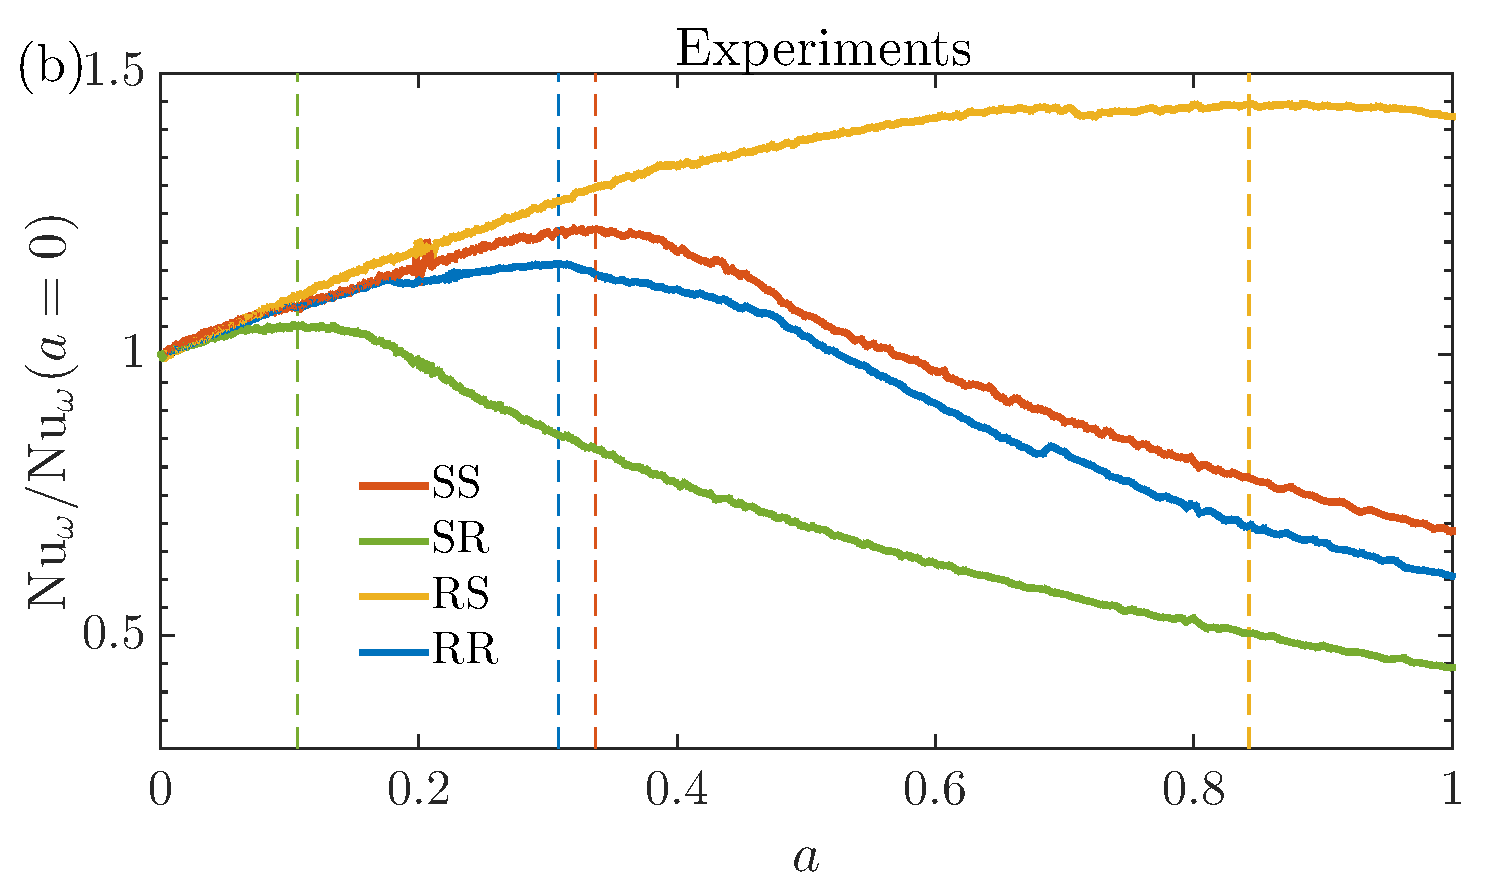
\includegraphics[width=3.2in]{3b.eps}
\caption{{\bf Optimal transport peak} $\Nu$ as a function of $a$ for constant driving strength, normalized by its value for $a=0$. {\bf a,} DNSs with $\Ta=1\times 10^9$. The optimal transport peaks are located at  $a_{opt,SS}=0.30$, $a_{opt,SR}=0.06$, $a_{opt,RS}=0.74$ and $a_{opt,RR}=0.28$. {\bf b,}  Experiments with $\Ta=4\times 10^{11} $. The optimal transport peaks for the 4 cases are located at $a_{opt,SS}=0.34$, $a_{opt,SR}=0.11$, $a_{opt,RS}=0.84$ and $a_{opt,RR}=0.31$. All optimal transport peaks are indicated by the dashed lines.}
\label{fig:Nu_a}
\end{center}
\end{figure}


%%%%%%%%%%%%%%%%%%%%
%%%%%% Energy dissipation %%%%	
%%%%%%%%%%%%%%%%%%%%

\begin{figure}[htbp]
     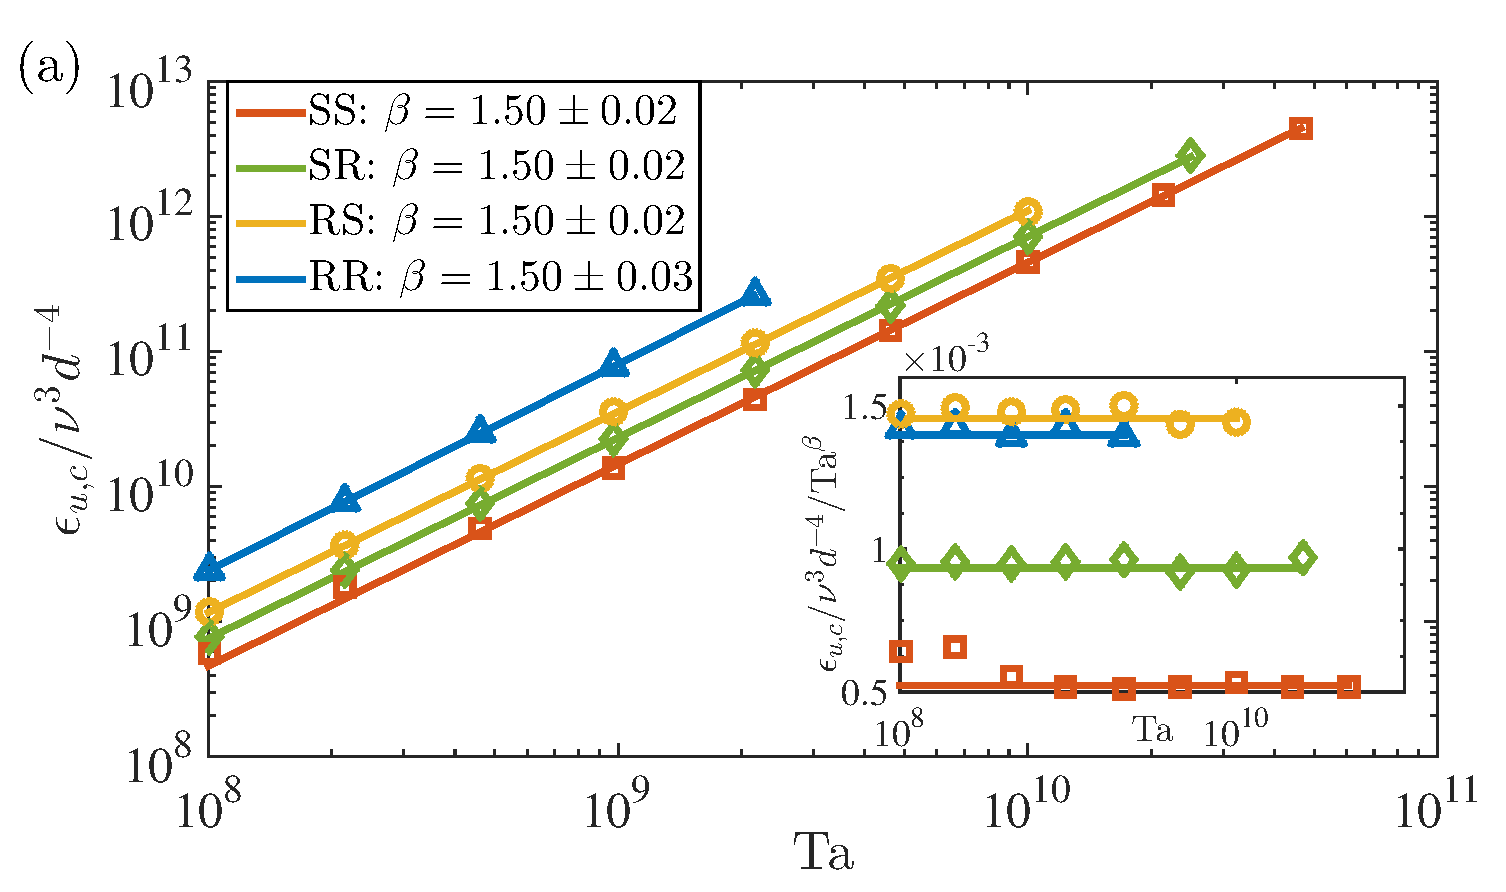
\includegraphics[width=3.2in]{5a.eps}
    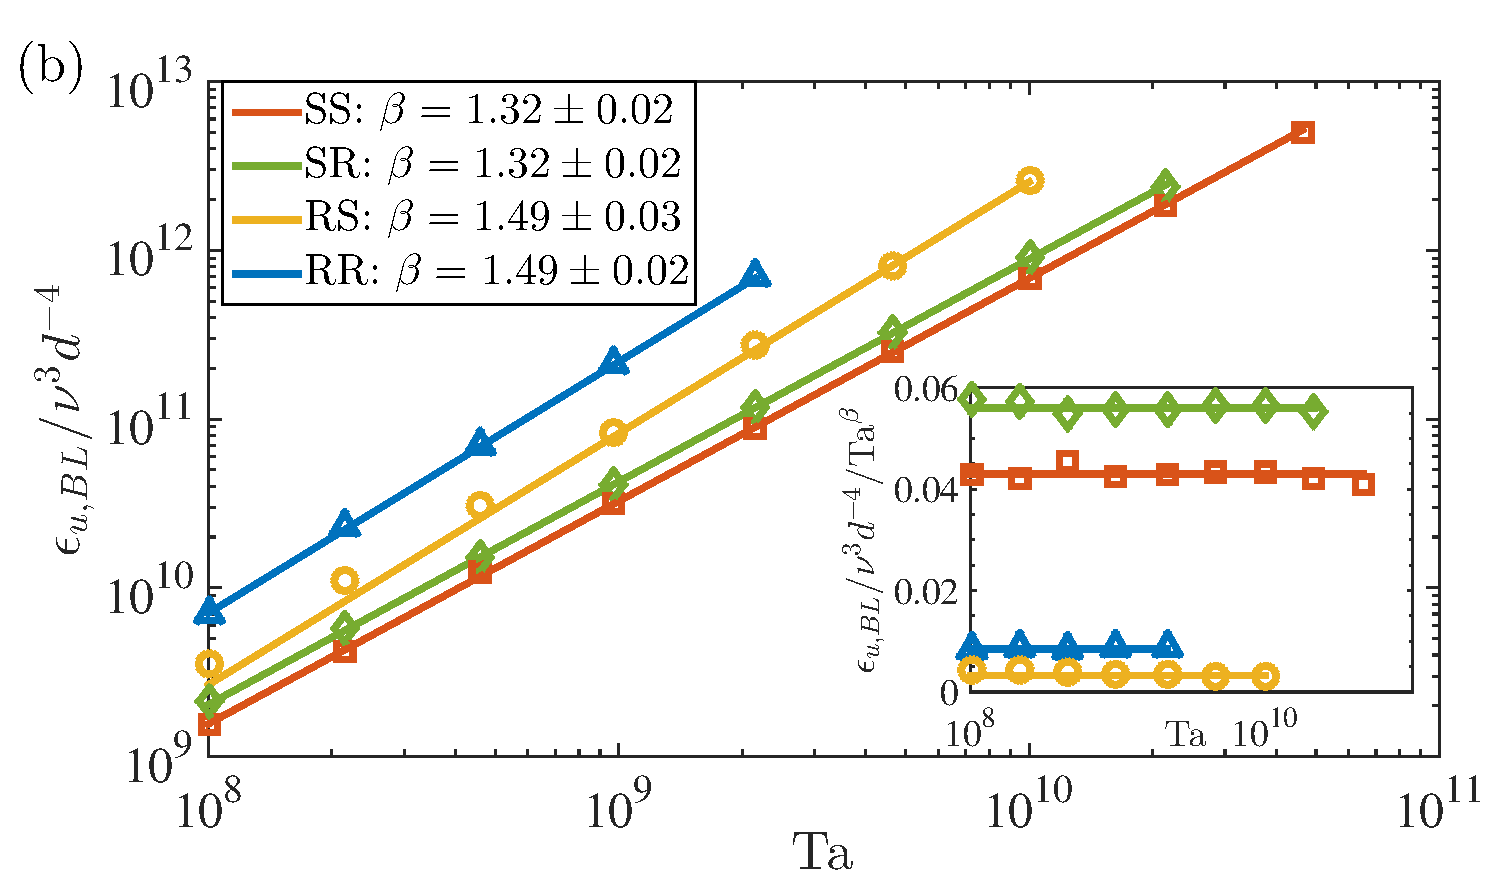
\includegraphics[width=3.2in]{5b.eps}
\caption{{\bf Local energy dissipation rate from simulations.} Local energy dissipation rate in the bulk $\epsilon_{u,c}$ (at the center of the gap, averaged over the height) and in the inner cylinder boundary layer $\epsilon_{u,BL}$ (averaged in the range of wall distance zero to the point of maximum root mean square of azimuthal velocity) as a function of $\Ta$. The symbols are  the same as in Fig.\ \ref{fig:fig2}. The lines show the best fits of them.\ {\bf a,} The bulk energy dissipation rate follows $\epsilon_{u,c} \sim \Ta^{1.50} \sim Re_i^3$, irrespective of whether the wall is smooth or rough.\ {\bf b,} The boundary layer dissipation rate follows $\epsilon_{u,BL} \sim \Ta^{1.32}$ for the cases with smooth walls while it scales with $\epsilon_{u,BL} \sim \Ta^{1.50}$ for cases with rough walls.}
\label{fig4}
\end{figure}


\section{Local flow organization and profiles} 

Till now, we have focused on the global transport properties, however, the details of boundary layer-bulk interaction, and in particular how the local scalings affect the global ones, are still unknown. To verify the theory mentioned before, we split the mean energy dissipation rate from our DNS data into boundary layer and bulk contributions, following the GL approach \cite{gro00,gro01}. In Fig.~\ref{fig4}(a), the local energy dissipation rates at mid-gap $\epsilon_{u,c}$  are shown as a function of $\Ta$ (only inner cylinder rotation). It is clear that no matter whether the wall is smooth or rough, the bulk energy dissipation rate follows $\epsilon_{u,c}\sim \Ta^{3/2} \sim 
\Re_i^3$, which corresponds to the asymptotic ultimate regime without any logarithmic correction. In analogy, for RB turbulence, the same scaling exponent $\epsilon_{u,c}\sim \Ra^{3/2}$ was reported in Refs.\ \cite{sha08,ni11b}. Therefore, the crucial element determining the overall scaling is the dissipation rate in the boundary layer. To further confirm this, we show the local energy dissipation rates of the boundary layer $\epsilon_{u,BL}$ (averaged in the range of wall distance zero to the point of maximum root mean square of azimuthal velocity) in Fig.~\ref{fig4} (b). For the case with smooth walls, we find $\epsilon_{u,BL} \sim \Ta^{1.32}$ because of the $\Re_i$ dependent velocity profile, while for the boundary layers at rough walls we have $\epsilon_{u,BL} \sim \Ta^{3/2}$ because, as shown above, roughness cancels out the $\Re_i$ dependence and thus restores the asymptotic ultimate regime scaling. 
The competition between the boundary layer and bulk
ultimately determines the global scalings.


%%%%%%%%%%%%%%%%%%%%
%%%%%% Velocity profiles % %%%%	
%%%%%%%%%%%%%%%%%%%%
\begin{figure}[!htp]
%\begin{center}
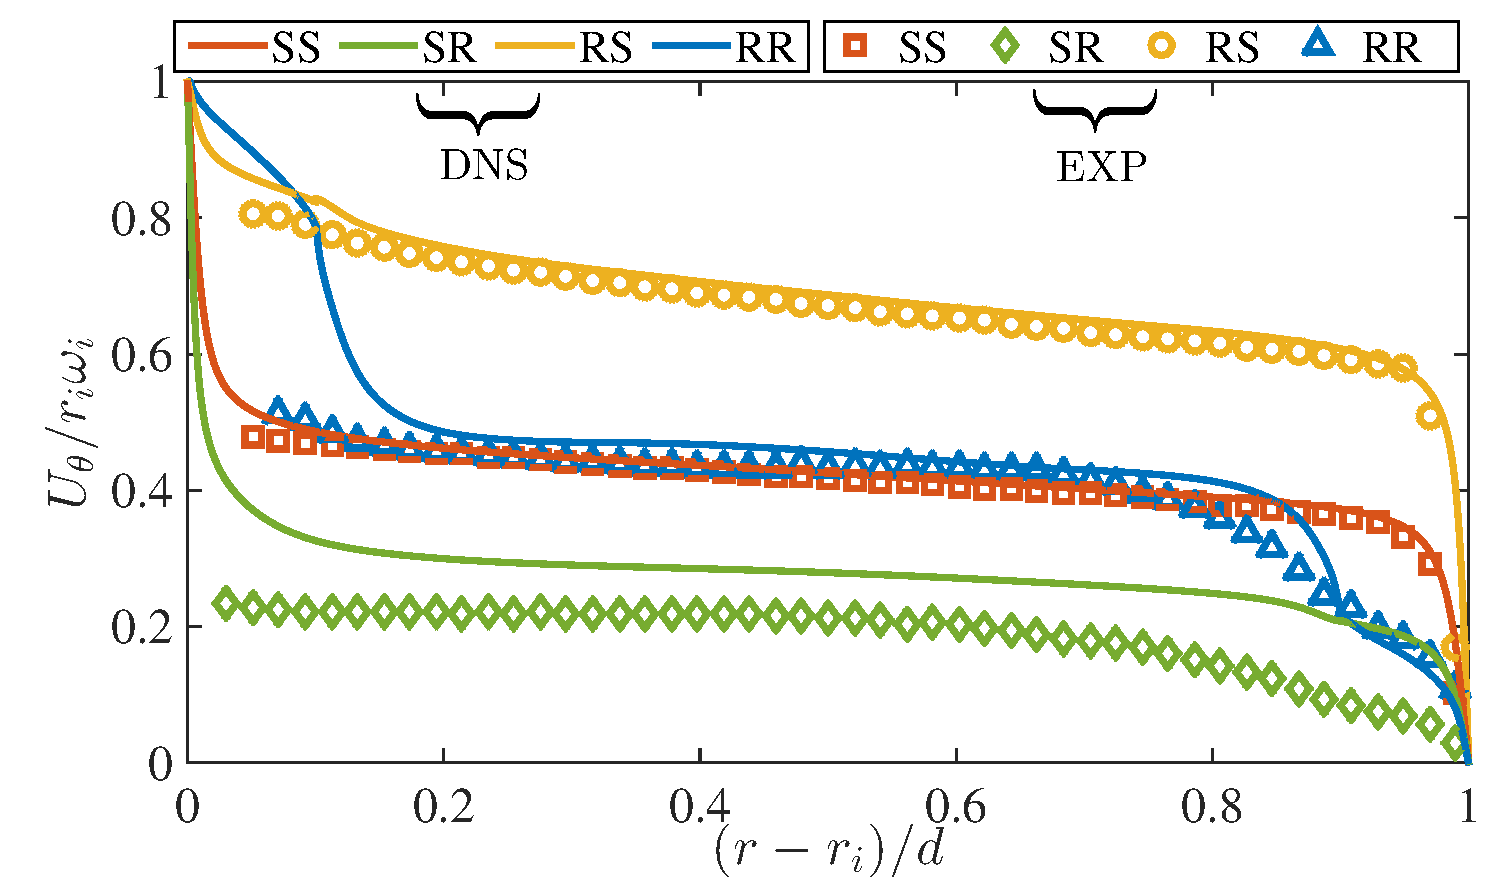
\includegraphics[width=3.2in]{4.eps}
\caption{{\bf Mean velocity profiles.} Normalized azimuthal velocity $U_{\theta}(r)/(r_i \omega_i)$ profiles as a function of the normalized radius $(r-r_i)/d$ for only inner cylinder rotation. Experimental and numerical data are shown in the same figure. EXP: $\Re_i = 5\times 10^5$ and DNS: $\Re_i = 3.74\times 10^4$. The experimental results were obtained using PIV.}
\label{fig:vel_prof}
%\end{center}
\end{figure}

From another point of view, roughness blocks the flow. Therefore, the main contribution to the torque comes from the pressure differences between the side surfaces of rough elements, rather than viscous forces. With roughness, we expect the shear rate close to the rough wall to decrease significantly, compared with the smooth case. This is clearly shown in Fig.\  \ref{fig:vel_prof}. With smooth cylinders, the normalized velocity profiles are characterized by a bulk region, in which the velocity is relatively constant ($U_{\theta}=0.45r_i \omega_i$). When a single cylinder is rough, the bulk velocity is completely dominated by the velocity of the rough cylinder, or in other words, bulk is enslaved by the rough wall. In the RR case, although the impact of roughness to the bulk flow balances, because that the torque is still dominated by pressure forces, the shear rate at the rough cylinder is also smaller as compared with the smooth case. The implication is that with roughness, a larger fraction of energy dissipates in the bulk, and thus the system is more bulk dominant. As mentioned before, the bulk energy dissipation rate follows $\epsilon_{u,c}\sim \Ta^{3/2}$, which implies the asymptotic ultimate regime. The more bulk is dominant, the closer the system reaches the ultimate regime without any logarithmic correction. This is indeed verified by the flow structure in Fig.\  \ref{fig:fig1}, where for the rough case, the plumes shedding from the roughness elements on one wall elongate towards the other wall and push more energy dissipation in the bulk compared to the smooth case.   


\section{Conclusions and outlook} 

Despite that in recent years various studies have been performed on turbulence with wall-roughness in closed systems, the results are highly scattered on the power law exponents between the transport and the driving forces \cite{cil99,she96,du00,roc01,ber03,tis11}, i.e. there is no consensus on whether asymptotic ultimate turbulence 1/2 power law, a concept that was postulated 50 years ago by R.\ Kraichnan \cite{kra62}, can be achieved or not \cite{ahl09}. In contrast, here with both strong experimental and numerical evidence, we demonstrate that the asymptotic ultimate regime exponent 1/2, the upper limit of transport, can be realized with the implementation of wall-roughness. The mechanism is that wall-exponent roughness eliminates the Reynolds number dependence of transport inside the boundary layer, thus helps to attain the asymptotic ultimate regime. The insights gained from this study provides valuable guidance for wall-bounded turbulence with wall-roughness in the ultimate regime in general, which is useful for a wide range of applications in industrial, geophysical, meteorological and oceanographical flows.



\newpage







\newpage



%%%%%%%%%%%%%%%%%%%%%%%%%%%%%%%%%%%%%%%%%%%%%%%%%%%%%%%%%%%%%%%%
%%%%%%%%%%%%%%%%%%%%%%%%      METHODS           %%%%%%%%%%%%%%%%%%%%%%%%%%%%%
%%%%%%%%%%%%%%%%%%%%%%%%%%%%%%%%%%%%%%%%%%%%%%%%%%%%%%%%%%%%%%%%
\newpage
\section{Methods}

%\annotation{The Methods section should be subdivided by short bold headings referring to methods used and we encourage the inclusion of specific subsections for statistics, reagents and animal models. If further references are included in this section, the numbering should continue from the end of the last reference number in the rest of the paper and the list should accompany the additional Methods at the end of the paper. The Methods section cannot contain figures or tables (essential display items should be included in the Extended Data).}


\subsection{Experimental methods}

\subsubsection{Experimental apparatus}
The experiments were performed in the Twente Turbulent Taylor-Couette facility (T$^3$C) \cite{gil11a}, consisting of two independently rotating concentric cylinders. The setup has an inner cylinder with a radius of $r_i=$ 200 mm and an outer cylinder with a radius of $r_o=$ 279.4 mm, resulting in a radius ratio of $\eta = r_i/r_o = 0.716$ and a gap width of $d=r_o-r_i=$ 79 mm. The gap is filled with water with a temperature of T $ \approx 20 ^{\circ}$C. In this work, the inner and outer cylinder rotate up to $\omega_i/2\pi=$ 7.5 Hz and $\omega_o/2\pi=$ 5 Hz, respectively, resulting in Reynolds numbers up to $\text{Re}_i = \omega_i r_i d/\nu = 7.5 \times 10^5$ and $\text{Re}_o= \omega_o r_o d/\nu = 7 \times 10^5$. The cylinders have a height of $L =$ 927 mm, resulting in an aspect ratio of $\Gamma = L/(r_o-r_i) = 11.7$. The end plates rotate with the outer cylinder.
The cylinders were made rough by attaching 6 vertical strips with a square cross-section ($6 \times 6$ mm, i.e.\ 7.5\% of the gap width) over the entire height on none, both or either one of the cylinders, similar as in ref.\ \cite{ber03, cad97} (Fig.\ \ref{fig:setup}). The roughness height is much larger than the boundary layer thickness \cite{hui13}. 

\begin{figure}[htp]
\begin{center}
\includegraphics[scale=1]{Rough_TC2.eps}
\caption{{\bf Experimental setup} (a) Schematic of the top view of both the experimental and numerical setup for the (RR) case, i.e. both cylinders rough. The six ribs (not to scale), which are perpendicular to the axis of rotation, have a square cross section and extend over the entire height of the cylinders. Their size is 7.5\% and 10\% of the gap width for the experiments and DNSs, respectively  (b) Vertical cross-section of the experimental setup, showing the position of the torque sensor and the PIV setup. For the PIV measurements, the laser illuminates the horizontal ($r, \theta$) plane at mid-height, $z = L/2$, see the Methods section.}
\label{fig:setup}
\end{center}
\end{figure}

\subsubsection{Torque measurements}
The torque is measured with a co-axial torque transducer (Honeywell 2404-5K, maximum capacity of 565 Nm), located inside the inner cylinder, to avoid measurement errors due to seals- and bearing friction, as shown in figure \ref{fig:setup}. In previous studies using this setup, the inner cylinder consisted of 3 different compartments, in which torque was measured in the middle section to exclude end plate effects \cite{gil11,gil12,hui14}. Here, we measure over the entire height of the cylinder, which accounts for the slightly different results for the SS case as compared to these studies.

\subsubsection{Velocity measurements}
Planar particle image velocimetry (PIV) measurements were performed in the $\theta-r$ plane at mid-height ($z=L/2$). We used a high-resolution sCMOS camera (pco.edge camera with 2560 px $\times$ 2160 px resolution), which was operated in double frame mode, as depicted in fig.\ \ref{fig:setup}. We record images through transparent windows in the bottom plate. The flow was illuminated from the side with a pulsed laser (532 nm Quantel Evergreen 145 Nd:YLF). The water was seeded with 20 $\mu$m fluorescent polymer particles (PMMA-RhB-10 by Dantec). The sheet thickness was approximately 1 mm. The PIV measurements were processed to give the averaged azimuthal velocity as a function of the radius $\langle u_{\theta}(r) \rangle_{\theta}$.



\subsection{Numerical methods}
The motion of the fluid is governed by the incompressible Navier-Stokes equations in the frame co-rotating with the outer cylinder
\begin{eqnarray}
\label{equ1}
\frac{\partial \bf{u}}{\partial t}+{\bf{u}} \cdot \nabla {\bf u} &=&- \nabla p + \frac{f(\eta)}{\Ta^{1/2}}{\nabla}^2 {\bf u}-\Ro^{-1}{\bf e }_z\times {\bf u }, \\
\nabla  \cdot {\bf u} &=& 0, 
\end{eqnarray}
where $\bf u$ and $p$ are the fluid velocity and pressure, respectively. $f(\eta)$ is a geometrical factor which is in the form 
\begin{eqnarray}
f(\eta)= \frac{(1+\eta)^3}{8\eta^2}.
\end{eqnarray}
$\Ta$ is the Taylor number and $\Ro$ the Rossby number which characterizes the strength of the driving force. The rotation ratio $a=-\omega_o/\omega_i$ is interchangeable with Rossby number through
\begin{eqnarray}
\Ro^{-1} =\frac{2\omega_o d}{|\omega_i-\omega_0|r_i}=-2\frac{1-\eta}{\eta}\frac{a}{|1+a|}.
\end{eqnarray}
The inner cylinder Reynolds number $\Re_i=r_i\omega d/\nu$ and outer cylinder Reynolds number $\Re_o=r_o\omega d/\nu$ are associated with $\Ta$ and $\Ro$ through
\begin{eqnarray}
\Re_i=\frac{\Ta^{1/2}} {f(\eta)} \left (1+\frac{\eta \Ro^{-1}}{2(1-\eta)}\right)
\end{eqnarray}
and
\begin{eqnarray}
\Re_o=\frac{\Ro^{-1}\Ta^{1/2}}{2f(\eta)(1-\eta)}.
\end{eqnarray}

The governing equations are solved using an energy conserving second-order finite-difference code \citep{ver96}, in combination with an immersed-boundary method \citep{fad00,yan06} to deal with the roughness. To achieve high performance computation, a two-dimensional MPI decomposition technique (MPI-pencil) \citep{poe15cf} is adopted. Weak and strong scaling tests show the linear behaviour of the code up to 64K cores. 
The code has been extensively validated and used for TC flow with smooth \cite{ost14pof, ost14pd, ost15pof} and rough \cite{zhu16,zhu17} walls. The axial direction is periodic and thus the end plate effects \cite{avi12} are eliminated. The radius ratio is chosen as $\eta=0.716$. The aspect ratio of the computational domain $\Gamma=L/d$, where $L$ is the axial periodicity length, is taken as $\Gamma=2.09$. When both walls are roughened, the inner and outer cylinder 
surfaces have six vertical ribs of square cross section
(edge width $h=0.1d$), respectively. The riblets are equi-distributed in the azimuthal
direction, similar to the experimental implementation. A rotational symmetry of order $n_{sym}=6$ is imposed to achieve a minimum azimuthal extent. The computation box is tested to be large enough to capture the sign changes of the azimuthal velocity autocorrelation at the mid-gap, as suggested as a criterion for the box size \cite{ost15pof}. Besides, the appropriate number of grid points
is chosen to make sure that enough resolution has been employed \cite{ost14pof,ost14pd}. E.g.\ at $\Ta=2.15\times10^9$ for the RR case, $3072\times1536\times1536$ grid points are used.


\subsection{Extention of Grossmann-Lohse theory with wall-roughness}

To explain the asymptotic ultimate scaling $1/2$ found in this manuscript, here we first recall the origin of the logarithmic correction. We take the case of only inner rotation as an example. According to the Grossmann-Lohse (GL) theory \cite{gro11}, the local dissipation rate in the turbulent boundary layer \cite{ll87} is given by 
\begin{eqnarray}\label{EQ10}
\epsilon_u(z)=u_\tau^3/(\kappa z), 
\end{eqnarray}
where $u_\tau=\sqrt  {\tau / (2\rho \pi r^2 L) }$ is the friction velocity, with $\rho$ is the fluid density, $\kappa$ the von K\'arm\'an constant, $r$ can be either the inner cylinder radius $r_i$ or the outer one $r_o$, and $z$ is the distance from the wall. $u_\tau$ is connected with the inner cylinder velocity $U=r_i\omega_i$ through the law of the wall \cite{sch00}, which is shown for TC turbulence in Refs. \cite{hui13,ost14pof} to obey 
\begin{eqnarray}\label{EQ3}
\frac{u_\tau}{U}=\frac{\kappa}{\mathrm{ln}(\Re_i   {u_\tau}/{U}  /{B})}.
\end{eqnarray}
$\Re_i$ is the inner cylinder Reynolds number and which for pure inner cylinder rotation can be related to $\Ta$ through the expression $\Ta=\frac{(1+\eta)^6}{64\eta^4}\Re_i^2$, $B$ is a constant depending on the system geometry. By averaging the local dissipation rate along the radius, we can estimate the mean dissipation rate as
\begin{eqnarray}\label{EQ4}
\epsilon_{u,m} &\sim& \frac{1}{d/2} \int_{0}^{d/2} \epsilon_u(z)dz    \nonumber\\
                       &=& \nu^3d^{-4}\Re_i^3 L(\Re_i)                                                                             \nonumber\\
                       &=& \nu^3d^{-4}\Re_i^3 \left( \frac{u_\tau}{U} \right)^3 \frac{2}{\kappa}\mathrm{ln}\left(\Re_i\frac{u_\tau}{U}\frac{1}{2}\right).
\end{eqnarray}
Here we assume that logarithmic boundary layer extends from the wall to the mid-gap. Usually how far the log-layer extends depends on $\Re_i$ and can be a small fraction of the gap width, but still for both TC and pipe flows, taking the half gap width or radius  is a reasonable approximation to derive the friction laws \cite{lat92,lew99,sch00,pop00}. The term ${\cal{L}}(\Re_i)= (u_\tau/U)^3 \mathrm{ln}(\Re_iu_\tau/U)$, depending on $Re_i$, is the logarithmic correction \cite{gro11}. Using the well known exact relation between $\epsilon_{u,m}$ and $\Nu$, namely $\epsilon_{u,m}=\nu^3 d^{-4}\Ta(\Nu-1)\left (\frac{\sqrt \eta}{(1+\eta)/2} \right)^8$ \cite{eck07b} and $\Ta\sim  \Re_i^2$, one obtains
 \begin{eqnarray}\label{EQ5}
\frac{\epsilon_{u,m}}{\nu^3d^{-4}} \sim \Re_i^3 {\cal{L}}(\Re_i)  \,\, \mathrm{and} \,\, \Nu \sim \Ta^{1/2}\ {\cal{L}}(\Re_i).                                                                       
\end{eqnarray}
with the logarithmic correction ${\cal{L}}(\Re_i)$ for both dissipation rate and torque scalings. It leads to a less steep increase of $\epsilon_u$ with increasing $\Re_i$ than in the Kolmogorov bulk which scales as $\Re_i^3$, and hence decreases the torque scaling between $\Nu$ and $\Ta$ from asymptotic ultimate scaling $1/2$ to the effective scaling 0.38 \cite{gro11,gil11,he12}, as mentioned before.  

With both walls roughened, the log-law in the fully rough regime ($u_\tau h/\nu>70$ \cite{sch00}; all our rough cases are in this regime) becomes
 \begin{eqnarray}\label{EQ6}
\frac{u_\tau}{U}=\frac{\kappa}{\mathrm{ln}(d/h/B)},                                                                    
\end{eqnarray}
as shown for turbulent TC flow with one rough boundary layer in Ref. \cite{zhu17}.  The momentum transfer between the wall and the fluid is accomplished by the shear, which in the fully rough regime occurs predominantly by the pressure forces on the side surfaces of the rough elements, rather than by viscous forces \cite{pop00}. That in the ultimate regime the kinematic viscosity $\nu$ is an irrelevant parameter, is reflected in the velocity profile (Eq.~(\ref{EQ6})) being  {\it{independent}} of $\Re_i$. Replacing the velocity profile from the smooth one to the rough one in Eqs.~(\ref{EQ10}, \ref{EQ3}, \ref{EQ4}), remarkably we find that the logarithmic correction term for $\epsilon_{u,m}$ turns into a \textit{constant} and thus its effect on the scaling exponent vanishes. The mean dissipation rate and torque thus now scale as
 \begin{eqnarray}\label{EQ7}
\frac{\epsilon_{u,m}}{\nu^3d^{-4}} \sim \Re_i^3  \,\, \mathrm{and} \,\, \Nu \sim \Ta^{1/2},                                                                       
\end{eqnarray}     
which explains the asymptotic ultimate regime scaling seen in Fig.~\ref{fig:fig2} for the RR case. In the RS case, the boundary layer at smooth wall depends on $\Re_i$ while boundary layer at rough wall is independent of it, the logarithmic correction is reduced but not totally canceled.  





%%%%%%%%%%%%%%%%%%%%%%%%%%%%%%%%%%%%%%%%%%%%%%%%%%%%%%%%%%%%%%%%
%%%%%%%%%%%%%%%%%%%%         Reference           %%%%%%%%%%%%%%%%%%%%%%%%%%%%%%%%
%%%%%%%%%%%%%%%%%%%%%%%%%%%%%%%%%%%%%%%%%%%%%%%%%%%%%%%%%%%%%%%%
%\bibliographystyle{/Users/lohsed/Documents/papers/sty-files/prsty_withtitle}
%\bibliography{/Users/lohsed/Documents/papers/bib-files/nanobubble_literatur}


%\annotation{Authors should be listed surname first, followed by a comma and initials of given names. Authors should be listed surname first, followed by a comma and initials of given names. Titles of all cited articles are required. Titles of articles cited in reference lists should be in upright, not italic text; the first word of the title is capitalized, the title written exactly as it appears in the work cited, ending with a full stop. Book titles are italic with all main words capitalized. Journal titles are italic and abbreviated according to common usage. Volume numbers are bold. The publisher and city of publication are required for books cited. (Refer to published papers in Nature for details.)
%References to web-only journals should give authors, article title and journal name as above, followed by URL in full - or DOI if known - and the year of publication in parentheses.References to websites should give authors if known, title of cited page, URL in full, and year of posting in parentheses.}

%\bibliography{literatur,TC_rough}
\bibliographystyle{prsty_withtitle} 

\bibliography{literatur}

%\bibliography{/Users/lohsed/Documents/papers/bib-files/literatur}  %% please leave this line



%%%%%%%%%%%%%%%%%%%%%%%%%%%%%%%%%%%%%%%%%%%%%%%%%%%%%%%%%%%%%%%%
%%%%%%%%%%%%%%%%%%%%          Acknowledgement        %%%%%%%%%%%%%%%%%%%%%%%%%%%%%
%%%%%%%%%%%%%%%%%%%%%%%%%%%%%%%%%%%%%%%%%%%%%%%%%%%%%%%%%%%%%%%%

\newpage



\noindent {\bf
Acknowledgements} 

We gratefully acknowledge V. Mathai for insightful discussions. We would like to thank G. W. Bruggert and M. Bos, as well as G. Mentink and R. Nauta for their technical support and D.P.M. van Gils and R. Ezeta for various discussions and help with the experiments. The work is financially supported by the Dutch Foundation for
Fundamental Research on Matter (FOM), the Netherlands Center for Multiscale Catalytic
Energy Conversion (MCEC), the Dutch Technology Foundation (STW) and a VIDI grant (No.\ 13477), all sponsored by the Netherlands
Organisation for Scientific Research (NWO).  We thank the Dutch Supercomputing Consortium
SurfSARA, the Italian supercomputer FERMI-CINECA through the PRACE Project
No. 2015133124 and the ARCHER UK National Supercomputing Service through the DECI Project 13DECI0246 for the allocation of computing time.
\\

\noindent{\bf
Author Contributions}
X.Z., S.G.H., R.A.V., R.V., C.S. and D.L. conceived the idea.
R.A.V. and D.B. performed the measurements. X.Z. performed the numerical simulations. X.Z. and R.A.V. analyzed the data. 
X.Z., R.A.V. and D.L. wrote the paper. 
R.V., C.S. and D.L. supervised the project. 
 All authors discussed the physics and proofread the paper. \\

\noindent{\bf
Author Information}
Reprints and permissions information is available at
www.nature.com/reprints. The authors declare no competing financial
interests. Readers are welcome to comment on the online version of the paper. 
%\annotation{Most probably, this will be inserted later on by Nature}
Correspondence and requests for materials should be addressed to
D.L. (d.lohse@utwente.nl) or C.S. (chaosun@tsinghua.edu.cn).



%%%%%%%%%%%%%%%%%%%%%%%%%%%%%%%%%%%%%%%%%%%%%%%%%%%%%%%%%%%%%%%%
%%%%%%%%%%%%%%%%%%%%%      Extended Data figures1-6 & table1           %%%%%%%%%%%%%%%%%%%
%%%%%%%%%%%%%%%%%%%%%%%%%%%%%%%%%%%%%%%%%%%%%%%%%%%%%%%%%%%%%%%%

 

\newpage
\iffalse
\section{Extended Data}



\begin{table}[!h]
\caption{\label{tab:one}Scaling exponents $\gamma$ and optimal transport peak $a_{opt}$ for the 4 roughness cases. The scaling exponents of the $\Nu \sim \Ta^{\gamma}$ scaling are given for the 5 measured $a$-values, its averaged value and the DNSs (with $a=0$). The DNS data and the experimental results for $a=0$, 0.2, and 0.4 are shown in figure \ref{fig:fig2}.}
\begin{ruledtabular}
\begin{tabular}{lllll}
Experiments & SS & SR & RS &RR\\
$\gamma(a=-0.2)$  &0.41$\pm$0.03   & 0.46$\pm$0.02 &   0.45$\pm$0.01  &  0.52$\pm$0.01\\
$\gamma(a=0$)   & 0.44$\pm$0.02  &  0.45$\pm$0.01  &  0.46$\pm$0.01  &  0.51$\pm$0.01\\
$\gamma(a=0.2)$ &   0.43$\pm$0.02   & 0.45$\pm$0.01 &  0.47$\pm$0.01   & 0.51$\pm$0.01\\
$\gamma(a=0.4)$  &  0.45$\pm$0.02 &  0.45$\pm$0.02  &  0.46$\pm$0.01 &   0.51$\pm$0.01\\
$\gamma(a=0.6)$   &  0.46$\pm$0.03  &  0.45$\pm$0.03  &  0.46$\pm$0.01  &  0.51$\pm$0.01 \\
$\gamma_{avg}$ & 0.44$\pm0.02$ & 0.45$\pm0.02$ & 0.46$\pm0.01$ & 0.51$\pm0.01$ \\ \hline
$\gamma(DNS)$ & 0.38$\pm0.02$ & 0.41$\pm0.01$ & 0.42$\pm0.01$ & 0.50 $\pm0.01$ \\ \hline

$a_{opt}(EXP)$ & 0.30 &  0.06 & 0.74 &  0.34 \\
$a_{opt}(DNS)$ & 0.34 &  0.11 & 0.84 &  0.31 \\

\end{tabular}
\end{ruledtabular}
\end{table}
\fi
\end{document}





